\documentclass{standalone}
\usepackage{tikz}
\usetikzlibrary{patterns, positioning}
\usepackage[sfdefault]{ClearSans} %% option 'sfdefault' activates Clear Sans as the default text font
\usepackage[T1]{fontenc}

\begin{document}
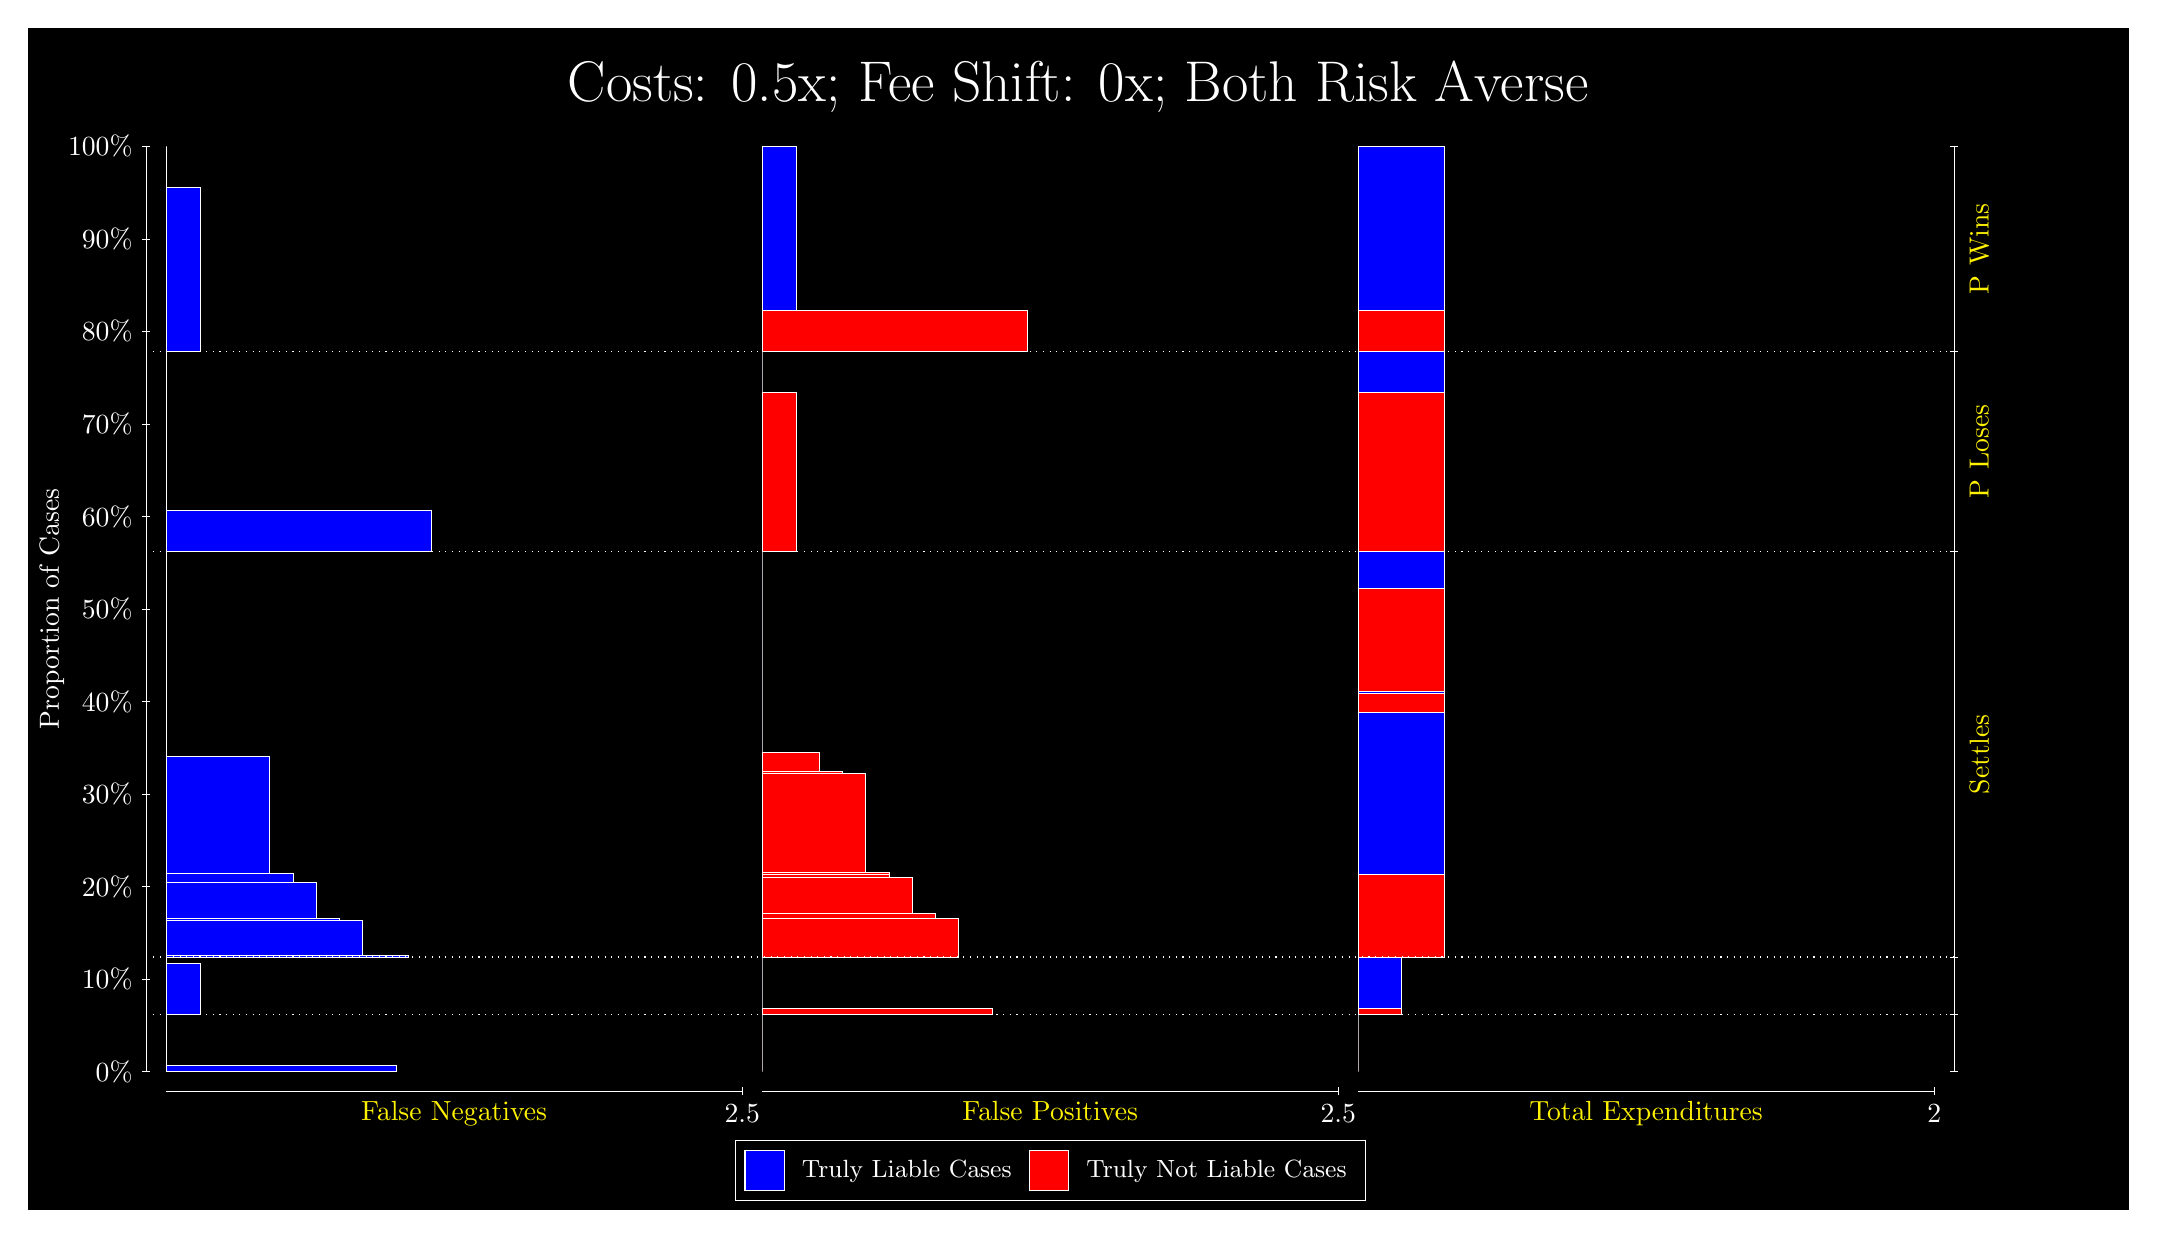
\begin{tikzpicture}
\draw[fill=black] (0,0) rectangle (26.667,15);
\draw[text=white] (0,13.5) rectangle (26.667,15) node[midway] {\huge Costs: 0.5x; Fee Shift: 0x; Both Risk Averse};
\draw[white, very thin] (1.5,1.75) -- (1.5,13.5);
\node[rotate=90, text=white, anchor=center] at (0.3, 7.625) {Proportion of Cases};
\draw[white, very thin] (1.45,1.75) -- (1.55,1.75);
\node[text=white, anchor=east] at (1.45, 1.75) {0\%};
\draw[white, very thin] (1.45,2.925) -- (1.55,2.925);
\node[text=white, anchor=east] at (1.45, 2.925) {10\%};
\draw[white, very thin] (1.45,4.1) -- (1.55,4.1);
\node[text=white, anchor=east] at (1.45, 4.1) {20\%};
\draw[white, very thin] (1.45,5.275) -- (1.55,5.275);
\node[text=white, anchor=east] at (1.45, 5.275) {30\%};
\draw[white, very thin] (1.45,6.45) -- (1.55,6.45);
\node[text=white, anchor=east] at (1.45, 6.45) {40\%};
\draw[white, very thin] (1.45,7.625) -- (1.55,7.625);
\node[text=white, anchor=east] at (1.45, 7.625) {50\%};
\draw[white, very thin] (1.45,8.8) -- (1.55,8.8);
\node[text=white, anchor=east] at (1.45, 8.8) {60\%};
\draw[white, very thin] (1.45,9.975) -- (1.55,9.975);
\node[text=white, anchor=east] at (1.45, 9.975) {70\%};
\draw[white, very thin] (1.45,11.15) -- (1.55,11.15);
\node[text=white, anchor=east] at (1.45, 11.15) {80\%};
\draw[white, very thin] (1.45,12.325) -- (1.55,12.325);
\node[text=white, anchor=east] at (1.45, 12.325) {90\%};
\draw[white, very thin] (1.45,13.5) -- (1.55,13.5);
\node[text=white, anchor=east] at (1.45, 13.5) {100\%};

\draw[white, very thin] (24.457,1.75) -- (24.457,13.5);
\draw[white, very thin] (24.407,1.75) -- (24.507,1.75);
\node[anchor=west] at (24.407, 1.75) {};
\draw[white, very thin] (24.407,2.4788) -- (24.507,2.4788);
\node[anchor=west] at (24.407, 2.4788) {};
\draw[white, very thin] (24.407,3.2049) -- (24.507,3.2049);
\node[anchor=west] at (24.407, 3.2049) {};
\draw[white, very thin] (24.407,8.3543) -- (24.507,8.3543);
\node[anchor=west] at (24.407, 8.3543) {};
\draw[white, very thin] (24.407,10.899) -- (24.507,10.899);
\node[anchor=west] at (24.407, 10.899) {};
\draw[white, very thin] (24.407,13.5) -- (24.507,13.5);
\node[anchor=west] at (24.407, 13.5) {};

\draw[white, very thin, fill=blue] (1.75,1.75) rectangle (4.6775,1.8267);
\draw[white, very thin, fill=red] (1.75,1.8267) rectangle (1.75,2.4788);
\draw[white, very thin, fill=blue] (1.75,2.4788) rectangle (2.1891,3.1295);
\draw[white, very thin, fill=red] (1.75,3.1295) rectangle (1.75,3.2049);
\draw[white, very thin, fill=blue] (1.75,3.2049) rectangle (4.8239,3.2247);
\draw[white, very thin, fill=blue] (1.75,3.2247) rectangle (4.5312,3.2279);
\draw[white, very thin, fill=blue] (1.75,3.2279) rectangle (4.2384,3.6751);
\draw[white, very thin, fill=blue] (1.75,3.6751) rectangle (3.9457,3.6992);
\draw[white, very thin, fill=blue] (1.75,3.6992) rectangle (3.6529,4.1508);
\draw[white, very thin, fill=blue] (1.75,4.1508) rectangle (3.3602,4.2721);
\draw[white, very thin, fill=blue] (1.75,4.2721) rectangle (3.0674,5.7516);
\draw[white, very thin, fill=red] (1.75,5.7516) rectangle (1.75,8.3543);
\draw[white, very thin, fill=blue] (1.75,8.3543) rectangle (5.1167,8.873);
\draw[white, very thin, fill=red] (1.75,8.873) rectangle (1.75,10.899);
\draw[white, very thin, fill=blue] (1.75,10.899) rectangle (2.1891,12.981);
\draw[white, very thin, fill=red] (1.75,12.981) rectangle (1.75,13.5);
\draw[white, very thin, fill=red] (9.3189,1.75) rectangle (9.3189,2.4021);
\draw[white, very thin, fill=blue] (9.3189,2.4021) rectangle (9.3189,2.4788);
\draw[white, very thin, fill=red] (9.3189,2.4788) rectangle (12.246,2.5541);
\draw[white, very thin, fill=blue] (9.3189,2.5541) rectangle (9.3189,3.2049);
\draw[white, very thin, fill=red] (9.3189,3.2049) rectangle (11.807,3.6992);
\draw[white, very thin, fill=red] (9.3189,3.6992) rectangle (11.515,3.7588);
\draw[white, very thin, fill=red] (9.3189,3.7588) rectangle (11.222,4.2221);
\draw[white, very thin, fill=red] (9.3189,4.2221) rectangle (10.929,4.2524);
\draw[white, very thin, fill=red] (9.3189,4.2524) rectangle (10.929,4.2858);
\draw[white, very thin, fill=red] (9.3189,4.2858) rectangle (10.636,5.5381);
\draw[white, very thin, fill=red] (9.3189,5.5381) rectangle (10.344,5.5676);
\draw[white, very thin, fill=red] (9.3189,5.5676) rectangle (10.051,5.8075);
\draw[white, very thin, fill=blue] (9.3189,5.8075) rectangle (9.3189,8.3543);
\draw[white, very thin, fill=red] (9.3189,8.3543) rectangle (9.758,10.38);
\draw[white, very thin, fill=blue] (9.3189,10.38) rectangle (9.3189,10.899);
\draw[white, very thin, fill=red] (9.3189,10.899) rectangle (12.686,11.418);
\draw[white, very thin, fill=blue] (9.3189,11.418) rectangle (9.758,13.5);
\draw[white, very thin, fill=red] (16.888,1.75) rectangle (16.888,2.4021);
\draw[white, very thin, fill=blue] (16.888,2.4021) rectangle (16.888,2.4788);
\draw[white, very thin, fill=red] (16.888,2.4788) rectangle (17.437,2.5541);
\draw[white, very thin, fill=blue] (16.888,2.5541) rectangle (17.437,3.2049);
\draw[white, very thin, fill=red] (16.888,3.2049) rectangle (17.986,4.2524);
\draw[white, very thin, fill=blue] (16.888,4.2524) rectangle (17.986,6.3184);
\draw[white, very thin, fill=red] (16.888,6.3184) rectangle (17.986,6.5584);
\draw[white, very thin, fill=blue] (16.888,6.5584) rectangle (17.986,6.5782);
\draw[white, very thin, fill=red] (16.888,6.5782) rectangle (17.986,7.8934);
\draw[white, very thin, fill=blue] (16.888,7.8934) rectangle (17.986,8.3543);
\draw[white, very thin, fill=red] (16.888,8.3543) rectangle (17.986,10.38);
\draw[white, very thin, fill=blue] (16.888,10.38) rectangle (17.986,10.899);
\draw[white, very thin, fill=red] (16.888,10.899) rectangle (17.986,11.418);
\draw[white, very thin, fill=blue] (16.888,11.418) rectangle (17.986,13.5);
\draw[white, dotted] (1.5,2.4788) -- (24.457,2.4788);
\draw[white, dotted] (1.5,3.2049) -- (24.457,3.2049);
\draw[white, dotted] (1.5,8.3543) -- (24.457,8.3543);
\draw[white, dotted] (1.5,10.899) -- (24.457,10.899);
\draw[white, very thin] (1.75,1.5) -- (9.0689,1.5);
\node[text=yellow, anchor=north] at (5.4094, 1.5) {False Negatives};
\draw[white, very thin] (9.0689,1.45) -- (9.0689,1.55);
\node[text=white, anchor=north] at (9.0689, 1.45) {2.5};

\draw[white, very thin] (9.3189,1.5) -- (16.638,1.5);
\node[text=yellow, anchor=north] at (12.978, 1.5) {False Positives};
\draw[white, very thin] (16.638,1.45) -- (16.638,1.55);
\node[text=white, anchor=north] at (16.638, 1.45) {2.5};

\draw[white, very thin] (16.888,1.5) -- (24.207,1.5);
\node[text=yellow, anchor=north] at (20.547, 1.5) {Total Expenditures};
\draw[white, very thin] (24.207,1.45) -- (24.207,1.55);
\node[text=white, anchor=north] at (24.207, 1.45) {2};



\node[text=yellow, centered, rotate=90] at (24.777, 5.7796) {Settles};
\node[text=yellow, centered, rotate=90] at (24.777, 9.6264) {P Loses};
\node[text=yellow, centered, rotate=90] at (24.777, 12.199) {P Wins};

\draw (12.978300999999998,1.5) node[draw=none] (baseCoordinate) {};
\begin{scope}[align=center]
        \matrix[scale=0.5, draw=white, below=0.5cm of baseCoordinate, nodes={draw}, column sep=0.1cm]{
            \node[rectangle, draw, minimum width=0.5cm, minimum height=0.5cm, fill=blue] {}; &
            \node[draw=none, font=\small, text=white] (B) {Truly Liable Cases}; &
            \node[rectangle, draw, minimum width=0.5cm, minimum height=0.5cm, fill=red] {}; &
            \node[draw=none, font=\small, text=white] (B) {Truly Not Liable Cases}; \\
            };
\end{scope}

\end{tikzpicture}
\end{document}